\chapter{Venerdì 19/03/2021}

\section{Traduzione dei nomi da C++ ad Assembler}
\paragraph{Cosa abbiamo visto fino ad ora?} Fino ad ora abbiamo affrontato questioni valide sia per il C che per il C++.
\paragraph{Overloading in C} Fino ad ora abbiamo introdotto le funzioni in questo modo
\begin{verbatim}
	extern "C" elab(...)
\end{verbatim}
indicare \emph{C} significa dire che la funzione rispetta lo standard del C. Nel C, ricordiamo, non è presente l'overloading e i nomi delle funzioni vengono tradotti esattamente come indicati nel codice.
\paragraph{Overloading in C++} L'overloading è presente in C++ e deve essere trattato. Possiamo avere funzioni con lo stesso nome, ma parametri in ingresso diversi (sia nel numero che nei tipi).
\begin{verbatim}
	elab(int)
	elab(int, int)
	elab(miastruct)
	elab(int*)
\end{verbatim}
queste sono funzioni diverse! Il compilatore, quando vede una chiamata del tipo
\begin{verbatim}
	elab(5)
\end{verbatim}
deve capire quale funzione chiamare. Ricordiamoci che due funzioni non si distinguono per il valore restituito: segue che non posso avere funzioni del tipo
\begin{verbatim}
	char elab(int)
	int elab(int)
\end{verbatim}
Se il compilatore sta compilando un file e nello stesso è presente la definizione di ciascuna di queste funzioni la cosa è semplice, mentre diventa più complessa se alcune funzioni (o tutte le funzioni) sono definite in altri files. Non posso indicare l'indirizzo della funzione, visto che non lo conosco: lascerò al collegatore le informazioni necessarie per capire quale funzione ci interessa. Il collegatore guarderà le tabelle dei simboli di tutti i files. 
\paragraph{In base a cosa stabilisco se l'etichetta è la stessa che sto cercando?} L'etichetta è una stringa, quindi mediante corrispondenza tra stringhe. 
\paragraph{Problema} Non posso definire più funzioni con la stessa etichetta \emph{elab}. Il collegatore vedrebbe più definizioni della stessa etichetta. Il problema nasce perché vogliamo utilizzare lo stesso collegatore del C.
\paragraph{Soluzione}  Modifichiamo i nomi posti delle etichette codificando all'interno gli argomenti della funzione. Dobbiamo individuare un algoritmo che produce la stessa stringa data la stessa funzione (ricordiamoci che il compilatore agisce sui singoli files in modo distinto).

\subsection{Regole per le etichette delle funzioni}
\paragraph{Osservazione} L'algoritmo non è standard. Esistono compilatori diversi con regole diverse.
\paragraph{Regole} Prendiamo una funzione
\begin{verbatim}
	funz(tipo1, tipo2, ..., tipoN)
\end{verbatim}
\begin{enumerate}
	\item La stringa inizia sempre così
	\begin{verbatim}
		_Z
	\end{verbatim}
	\item Segue il nome della funzione, preceduto dal numero di caratteri del nome (devo sapere quando si inizia a parlare dei tipi nella stringa)
	\begin{verbatim}
		4funz
	\end{verbatim}
	\item Segue la traduzione di ognuno dei tipi
	\begin{verbatim}
		_Z4funzS1S2...SN
	\end{verbatim}
\end{enumerate}
\paragraph{Quali sono i possibili tipi nel C++?} Il numero di tipi è piuttosto alto: abbiamo 
\begin{itemize}
	\item i tipi base (char, bool, int, long, unsigned/signed ....)
	\item i tipi definiti dall'utente (enum, class, struct...)
	\item i tipi composti (*,\&, const, array...)
\end{itemize}
\subsubsection{Tipi base} Per ogni tipo base c'è una lettera identificativa
\begin{center}
	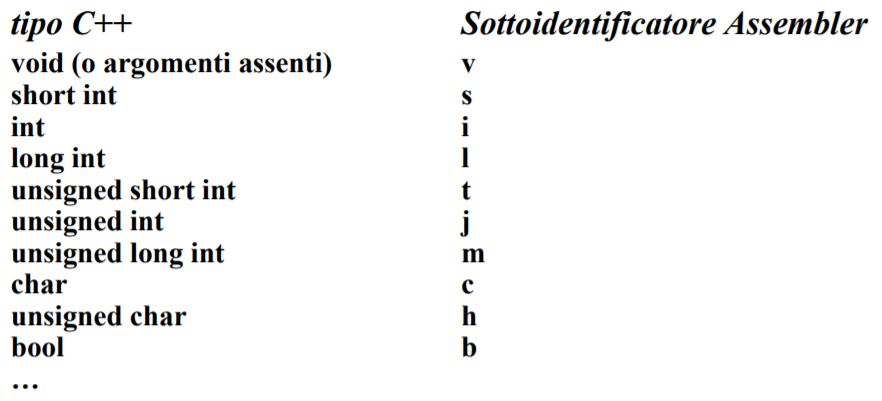
\includegraphics[scale=0.70]{img/38.PNG}
\end{center}  
notare che in assenza di argomenti è presente la lettera \emph{v} (\emph{void}). In presenza di più argomenti relativi a tipi base si pongono più caratteri in sequenza
\begin{verbatim}
	funz() ---> _Z4funzx
	funz(int) --->_Z4funzi
	funz(long int) ---> _Z4funzl
	funz(short int) ---> _Z4funzs
	funz(int, int) ---> _Z4funzii
\end{verbatim}
\subsubsection{Struttura} Supponiamo di voler trovare la stringa relativa a questa funzione
\begin{verbatim}
	funz(miastrutt)
\end{verbatim}
Trattiamo la cosa in modo simile al nome della funzione. \emph{miastrutt} ha nove caratteri, quindi
\begin{verbatim}
	_Z4funz9miastrutt
\end{verbatim}
Vediamo un ulteriore esempio che combina una struttura e un tipo base
\begin{verbatim}
	funz(mias, int, char)  ----> _Z4funz4miasic
\end{verbatim}
\subsubsection{Puntatori}
Poniamo P seguito dal tipo
\begin{verbatim}
	tipo* ----> PStipo
\end{verbatim}
Vediamo alcuni esempi
\begin{verbatim}
	int* ---> Pi
	mias* ---> P4mias
	int** --->  PPi
\end{verbatim}
\subsubsection{Riferimenti}
Poniamo R seguito dal tipo 
\begin{verbatim}
	tipo& ---> RStipo
\end{verbatim}
Vediamo alcuni esempi
\begin{verbatim}
	int& ---> Ri
	mias*& ---> RP4mias
\end{verbatim}
\subsubsection{Costanti}
Sulle costanti dobbiamo fermarci un attimo
\begin{verbatim}
	(1) const int*
	(2) int const* ---> Pki
	(3) int* const 
\end{verbatim}
Quanti tipi diversi ho dichiarato? Due:
\begin{itemize}
	\item Puntatore a intero costante (1 e 2, posso modificare l'indirizzo puntato ma non il valore dell'intero puntato)
	\item Puntatore costante a intero (3, posso modificare il valore dell'intero ma non l'indirizzo puntato)
\end{itemize}
\emph{const} si traduce con una K maiuscola. Nel capire di quale puntatore stiamo parlando dobbiamo ricordarci che \textbf{il \emph{const} fa sempre riferimento a ciò che è prima, tranne quando è in cima (in quel caso fa riferimento a ciò che viene dopo)}.
\paragraph{Regola della spirale} La regola della spirale (suggerimento mio, non di Lettieri) permette di capire in modo più facile di quale puntatore stiamo parlando:
\begin{itemize}
	\item parto dal nome dell'elemento;
	\item mi sposto indietro facendo un giro in senso orario (se becco la keyword \emph{const} devo contare fino a tre, e guardare a chi fa riferimento \underline{usando la regola di prima});
	\item ripeto fino al termine dell'espressione.
\end{itemize}
\begin{center}
	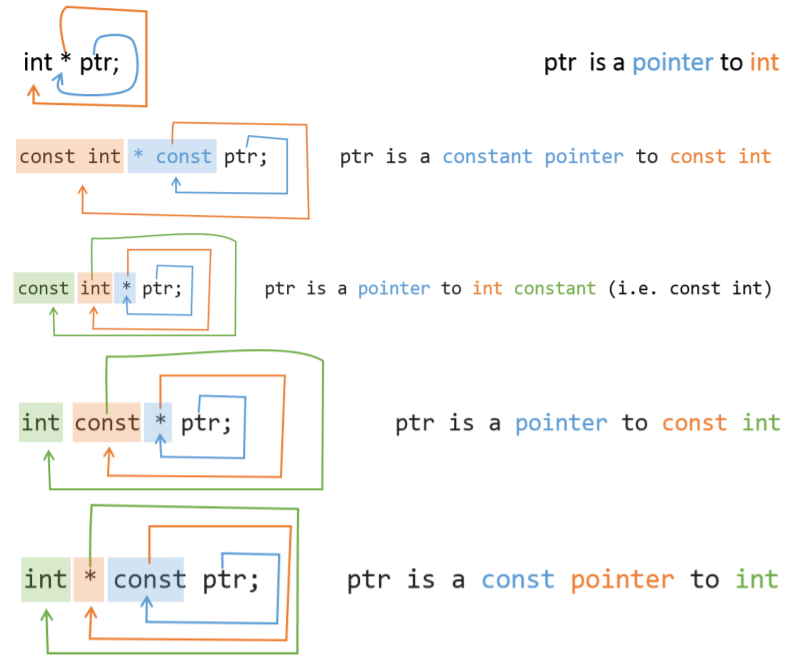
\includegraphics[scale=0.80]{img/154.PNG}
\end{center}  

\paragraph{Confronto tra tipi e tipi costanti nei parametri} Attenzione alle seguenti funzioni
\begin{verbatim}
	funz(int)
	funz(const int)
\end{verbatim}
non sono due funzioni diverse. Entrambe generano come stringa \begin{verbatim}_Z4funzi\end{verbatim}Nel secondo caso dico che non posso modificare la cosa che mi viene passata, ma succede la stessa cosa anche nel primo caso visto che si ha un passaggio per valore. Il ragionamento è valido anche parlando in modo generico.\paragraph{Conseguenza} In \emph{KPi} la lettera K non dice sostanzialmente niente, può essere tolto.
\[\boxed{\text{Se nel costruire l'etichetta pongo un \emph{K} all'inizio allora possiamo toglierlo}}\]
\subsubsection{Array}
Prendiamo i seguenti esempi
\begin{verbatim}
	f(int a[10])
	f(int a[100])     -------------> _Z1fPi
	f(int a[])
\end{verbatim}
sono le stesse funzioni, il numero non entra a far parte del nome della funzione. Inoltre, la seguente funzione è uguale alle precedenti
\begin{verbatim}
	f(int* a)          -------------> _Z1fPi
\end{verbatim}
Ricordiamo che passare un array come parametro significa passare un puntatore al primo elemento dell'array. Il fatto che un array decada in puntatore è una delle cose più criticate del C, conseguentemente anche del C++.\begin{framed}\noindent \textbf{Osservazione}: non affronteremo la regola per scrivere le etichette a riguardo, ma dobbiamo tenere a mente che funzioni di questo tipo non sono equivalenti
	\begin{verbatim}
		f(int a[][10])
		f(int a[][20])
	\end{verbatim} 
	possiamo mantenere implicita solo la prima dimensione, quella successiva no. Devo conoscere quanti interi sono presenti in ogni elemento dell'array, altrimenti non saprei come raggiungerli. Raggiungo l'elemento $a[i][j]$ con la seguente formula
	\begin{verbatim}
		i*secondaDim+j
	\end{verbatim}
\end{framed}

\subsubsection{Esempi di etichette con costanti}
\begin{itemize}
	\item Per ogni esempio
	\begin{itemize}
		\item Metto il solito inizio
		\item Per il nome pongo \emph{1f}
	\end{itemize}
	\item \begin{verbatim}
		f(int const*)   ----->  _Z1fPKi
	\end{verbatim}
	\begin{itemize}
		\item Per il tipo pongo \emph{PKi}: abbiamo un puntatore a un intero costante
	\end{itemize}
	\item \begin{verbatim}
		f(const int*)   ----->  _Z1fPKi
	\end{verbatim}
	\begin{itemize}
		\item Ricordiamoci la regola detta prima. L'etichetta ottenuta è la stessa della funzione precedente
	\end{itemize}
	\item \begin{verbatim}
		f(int* const)   ----->  _Z1fKPi   ----->  _Z1fPi
	\end{verbatim}
	\begin{itemize}
		\item Per il tipo pongo \emph{Pi}: abbiamo un puntatore costante a intero, abbiamo già detto che non ha senso mettere prima \emph{K}
	\end{itemize}
	\item \begin{verbatim}
		f(int const* const)   ----->  _Z1fKPKi   ----->  _Z1fPKi
	\end{verbatim}
	\begin{itemize}
		\item Per il tipo pongo \emph{PKi}: abbiamo un puntatore costante a intero costante. La \emph{K} prima non ha senso, quella dopo P invece è necessaria.
	\end{itemize}
	\item \begin{verbatim}
		f(int* const*)   ----->  _Z1fPKPi
	\end{verbatim}
	\begin{itemize}
		\item Per il tipo pongo \emph{PKPi}: abbiamo un puntatore a puntatore costante di intero.
	\end{itemize}
	\item \begin{verbatim}
		f(int*)   ----->  _Z1fPi
	\end{verbatim}
	\begin{itemize}
		\item Per il tipo pongo \emph{Pi}: abbiamo un puntatore a intero
	\end{itemize}
\end{itemize}
\begin{center}
	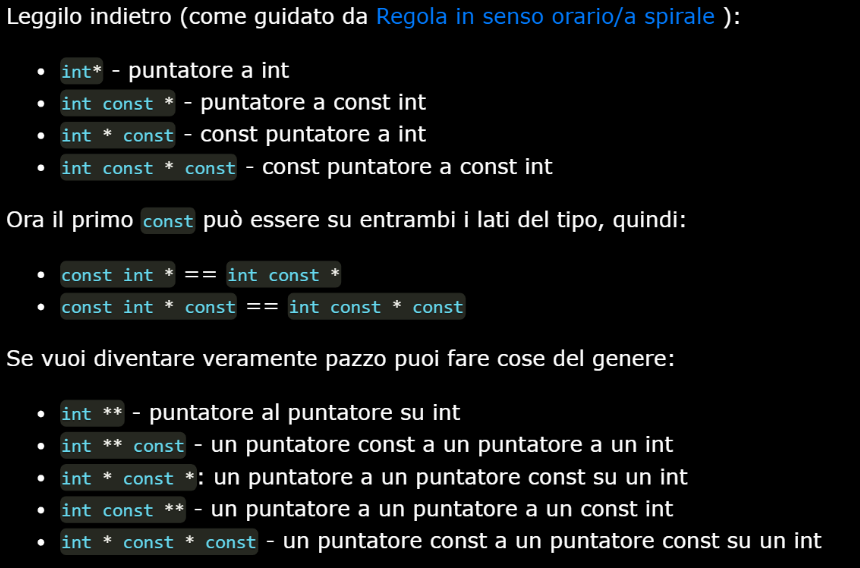
\includegraphics[scale=0.80]{img/155.PNG}
\end{center} 

\begin{framed}\noindent \textbf{Curiosità sui puntatori}. L'elemento $a[i]$ viene tradotto nel seguente modo
	\begin{verbatim}
		*(a+i)
	\end{verbatim}
	questa cosa è talmente vera in C, e quindi in C++, che possiamo dire
	\begin{verbatim}
		*(i+a)
	\end{verbatim}
	segue che dire
	\begin{verbatim}
		i[a]
	\end{verbatim}
	equivale a dire $a[i]$. La notazione è utilizzabile senza alcun problema in C e in C++.\end{framed}
